\section{The \instrument{} Instrument}
\label{sec:instrument}

\red{\textit{Instrument overview, description of instrument modes, etc.}}

\begin{figure}[!tb]
  \begin{center}
    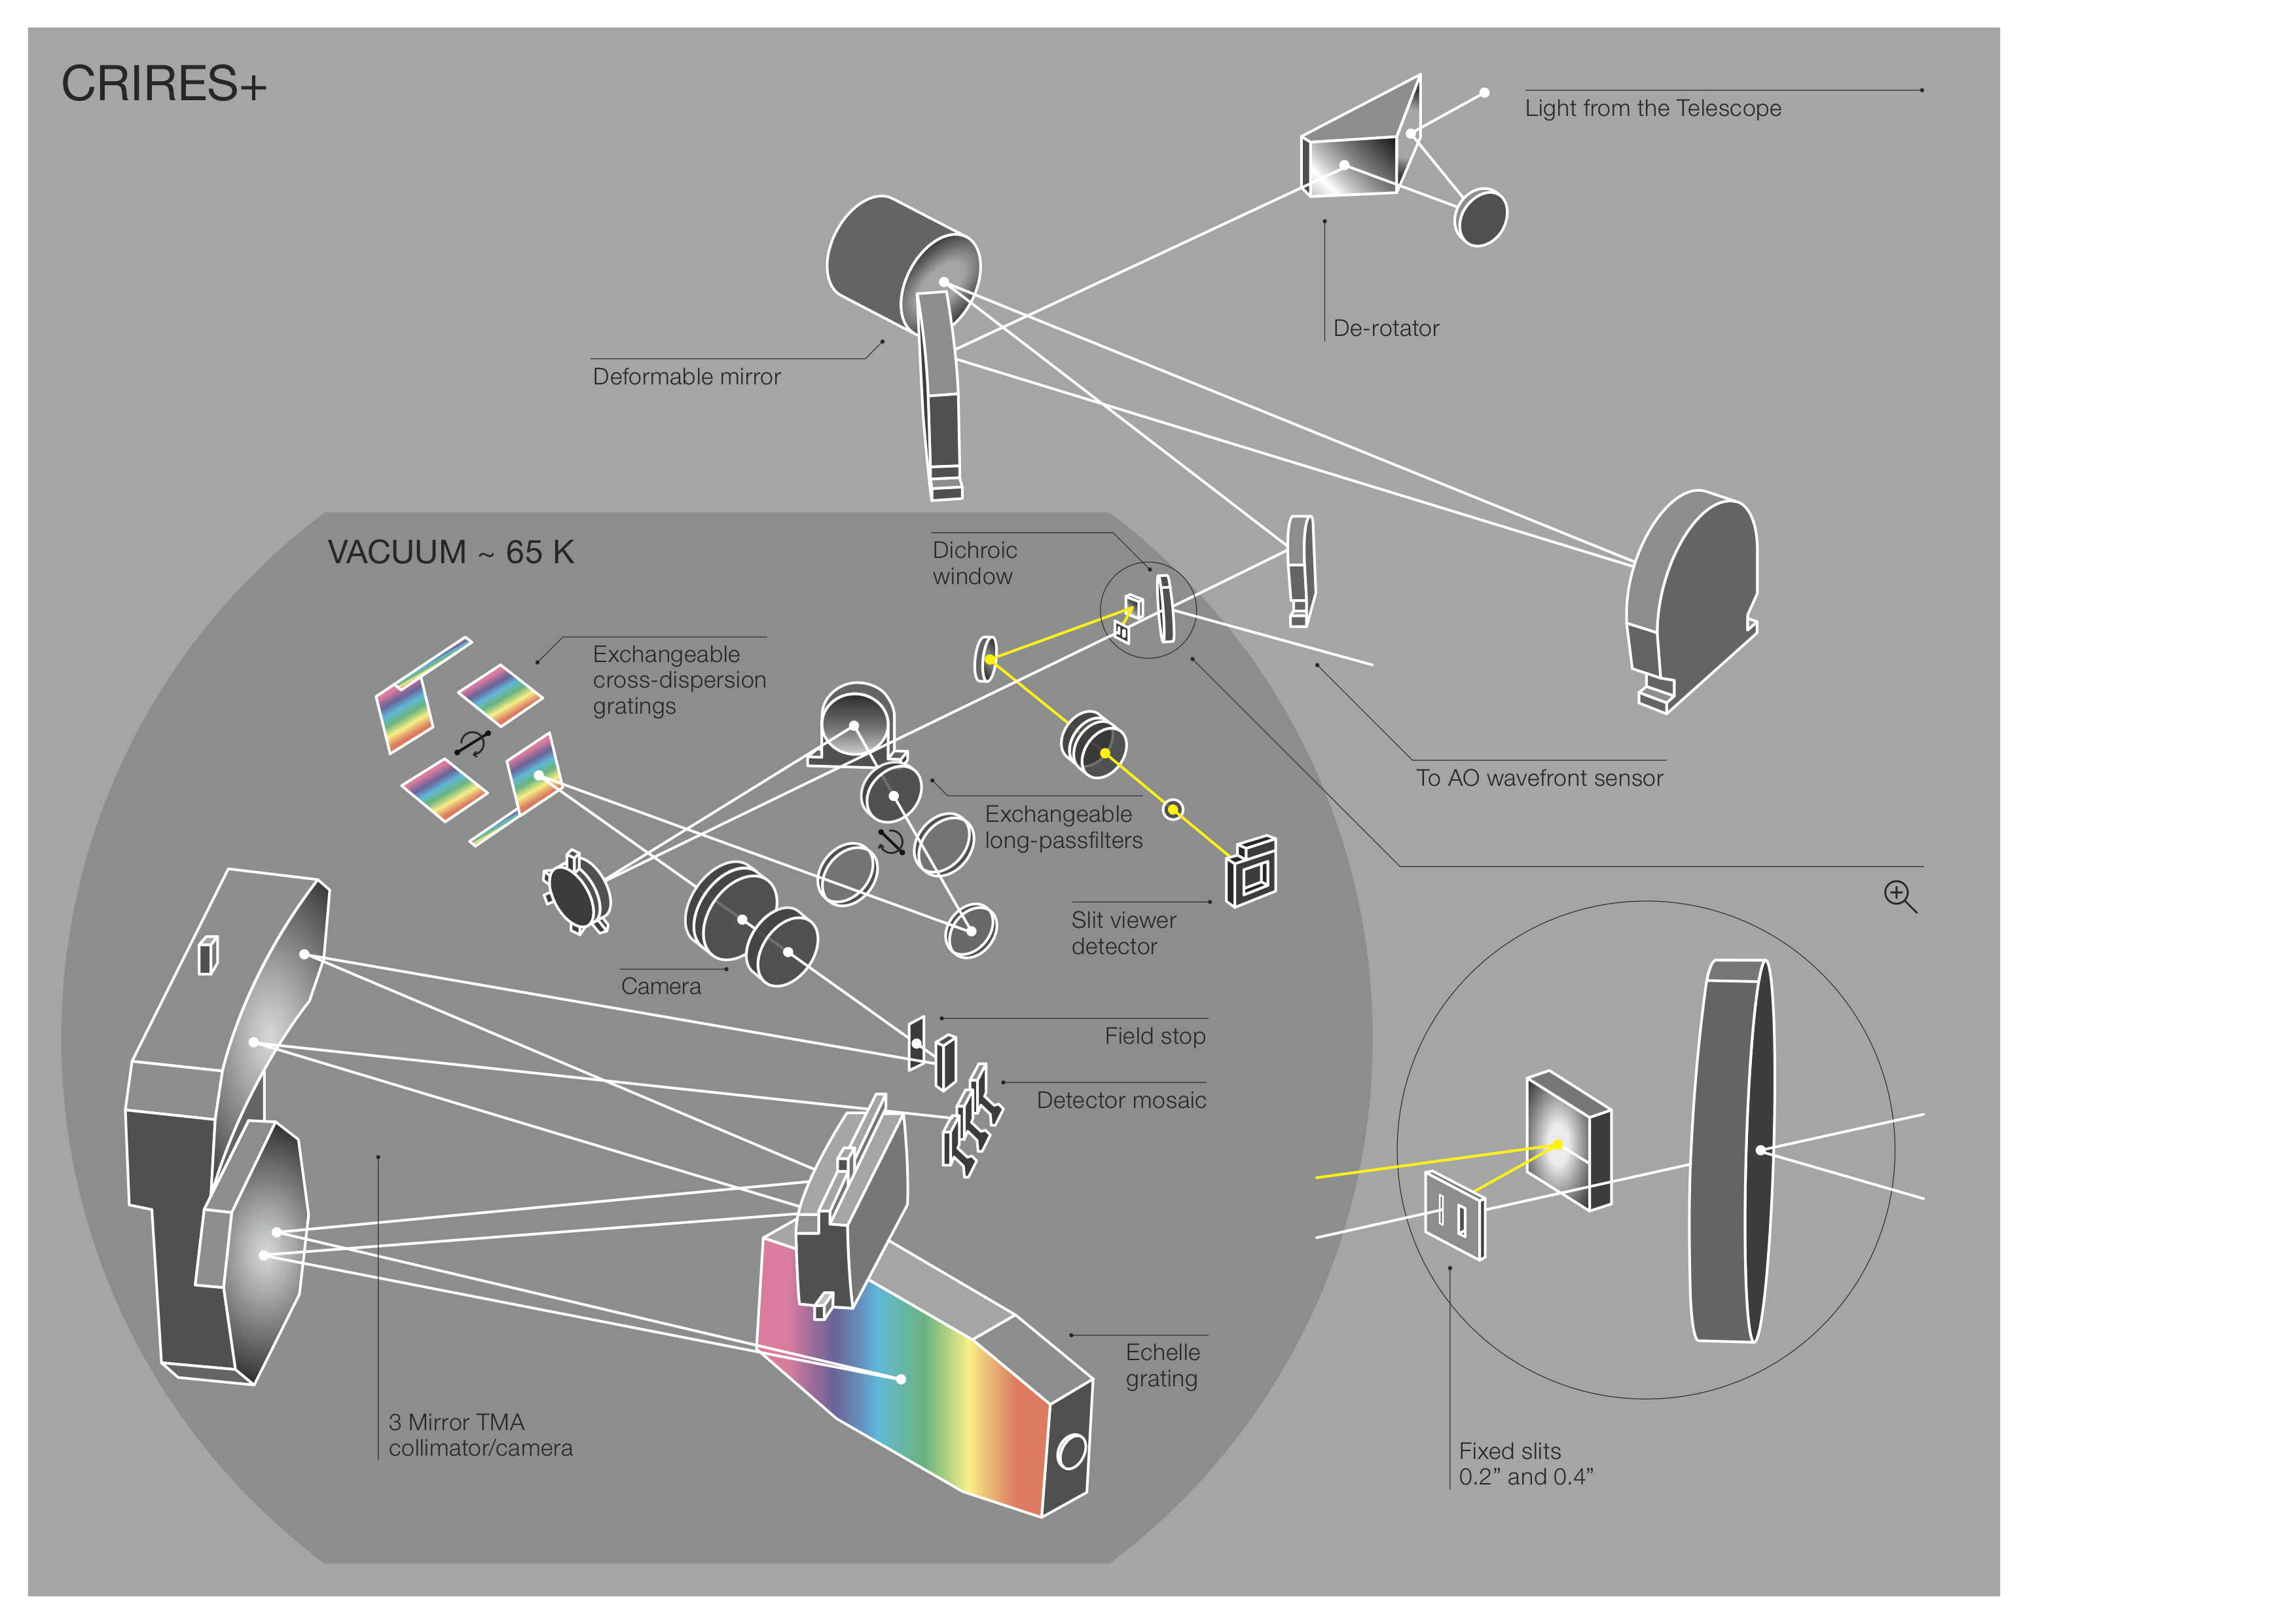
\psfig{file=figures/cr2res_instrument.jpg,width=0.75\linewidth}
  \end{center}
  \caption{
    \label{fig:cr2res_instrument}
    Graphical representations of \instrument{}.}
\end{figure}

%%% Local Variables:
%%% mode: latex
%%% TeX-master: t
%%% End:

